\section{Data analysis}
\label{sec:data-analysis}

\subsection{Pre-selection of laser data}
For each sensor, we selected a combination of angles and laser rings (for the Velodyne) or beams (for the others) that had a clear view of the snow-covered ground surface. The actual details for each sensor are given in Tab.~\ref{tab:selectionScans}. The range of the ground in our scans was between $x$=\SI{15}{\meter} to $x$=\SI{22}{\meter}. To simplify analysis, we considered as a snowfall echo any measurement which had a range reading of $x<$\SI{14.5}{\meter}. As will be shown later in section~\ref{subsub:Histo}, this is a valid approximation as the vast majority of those events happened for $x<$\SI{10}{\meter}. Thus, any snowflakes echoes between  $x>$\SI{14.5}{\meter} and the snow-covered ground surface are negligible, for all four sensors.

\begin{table*}[htbp]
    \centering
    % \def\tabularxcolumn#1{m{#1}}
    \begin{tabular}{|c|c|c|c|c|}
        \hline
        \textbf{Sensor}            & \textbf{Acquisition Frequency}  & \textbf{Selected beams/angles}  & \textbf{Selected rings}  & \textbf{Window size} \\\hline
        SICK LMS-200               & \SI{9.375}{\Hz}                      & 55 to 115                                    & N/A                         & ~\SI{106}{\second}       \\\hline
        SICK LMS151               & \SI{25}{\Hz}                           & 310 to 220                                  & N/A                         & ~\SI{40}{\second}        \\\hline
        Hokuyo UTM-30LX-EW  & \SI{20}{\Hz}                          & 440 to 590                                  & N/A                         & ~\SI{100}{\second}     \\\hline
        Velodyne HDL-32E        & \SI{10}{\Hz}                          & -0.05 to 0.25 $rad$                     & 17 to 31                   & ~\SI{40}{\second}      \\\hline
    \end{tabular}
    \caption{Details for data used in analysis. The Window size is the temporal window used to calculate statistics during the temporal evolution of a storm.}
    \label{tab:selectionScans}
\end{table*}

% ========================= Timing  ===================

\subsection{Temporal analysis}
A snowfall is a highly dynamic process, with large variation in snowing rates over its duration. Moreover, the snow physical characteristics (size, shape or reflectance) might vary significantly during a storm, affected by ambient conditions such as humidity level and temperature. Also, wind gusts might pull snow back up in the air or drive it sideways, affecting its effective fall rate. Consequently, one expect during a snowstorm to see significant short, medium and long term variations in the fraction of LiDAR echoes corresponding to the falling snow. 

Computing and reporting the temporal statistics for every scan would put too much emphasis on the very short-term statistics. Indeed, the inter-scan variation in the fraction of snowflake echoes can be significant. To better illustrate the process, we have overlaid four consecutive scans in the same plot for the LMS200 and for the first echo returned by the multi-echo Hokyyo sensor in Fig.~\ref{fig:LMS200_4Scans_Feb19}, for an intense snowing episode from the 02-19 data set. In these figures, we can see both the spatial and temporal variations of the echoes in snowflakes, which we suspect can be best described by a random process. For the discussion at hand, one can see a fluctuation in the fraction of echoes in snowflakes between scans, reported in the brackets of the legend. 

To smooth out these very short-term fluctuations, statistics are extracted from a number of consecutive scans contained in a time window of around 1~minute (detailed values in Tab.~\ref{tab:selectionScans}). Fig.~\ref{fig:TimingSnow}, shows this smoothed fraction of snowflakes echos compared to all returned laser measurements as a function of time, for the six snowiest days of our dataset. To allow for better visualization, only the LMS-200 and the Hokuyo's $1^{st}$ echo are plotted at their actual scale (1x): Others have been scaled up (from 30x to 200x), with their corresponding scaling factors reported in the legend. 

 \begin{figure}[th]
    \centering
    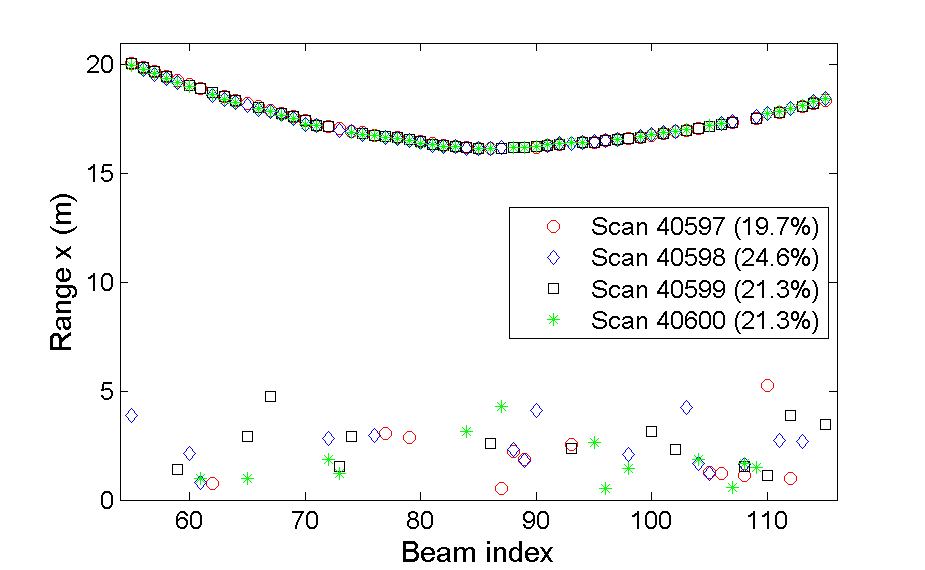
\includegraphics[width=0.95\linewidth]{./img/LMS200_4Scans_Feb19.png}
    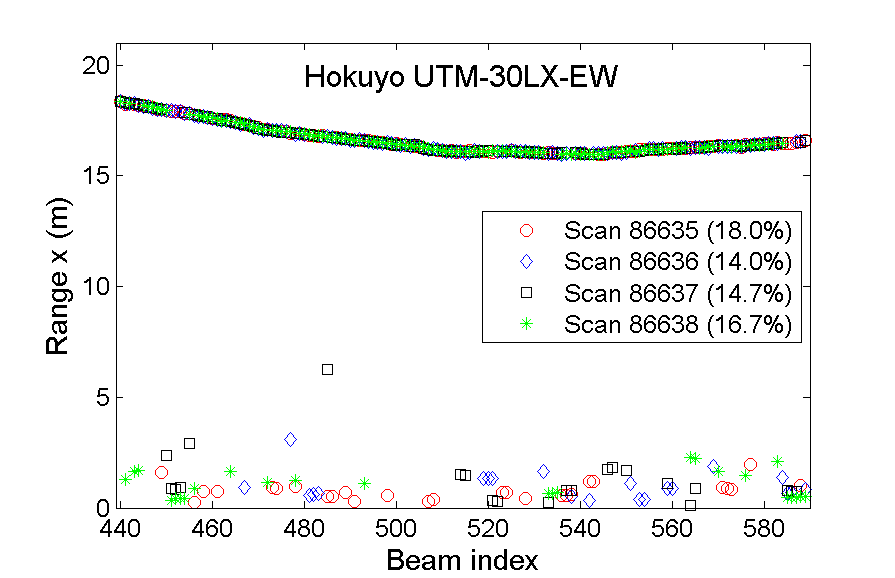
\includegraphics[width=0.95\linewidth]{./img/Hokuyo_4Scans_Feb19.png}
    \caption{Four overlaid consecutive scans for the LMS200 sensor (top), and the $1^{st}$ echo scans for the Hokuyo sensor (bottom), taken from the 02-19 dataset. Each symbol correspond to a particular scan. The curved line at the top corresponds to the snow surface on the ground. One can see the rapid variation of the snowflake echoes between scans, and how they are mostly limited to a range $x<$\SI{5}{\meter}. The percentage (in brackets) are the proportion of those echoes in the snowflakes.}
    \label{fig:LMS200_4Scans_Feb19}
\end{figure}

\subsubsection{SICK Sensors LMS-200 and LMS-151}
Our first conclusion based on Fig.~\ref{fig:TimingSnow} is that some sensors are more sensitive than others. The most sensitive device was the older LMS200, first introduced in the mid-2000. For the most intense snowstorms (Fig.~\ref{fig:TimingSnow}. b) 02-19, d) 03-17, e) 03-21 and f) 03-30), it peaked at around 15\%, for averaging windows of \SI{106}{\second}. As an older-generation device, it probably used unsophisticated algorithms and sensing. Indeed, its technical description~\cite{LMS200Manual} indicates that ``Raindrops and snow-flakes are cut out using pixel-oriented evaluation'', but this seems only applicable to  obstacle detection (field computation), not the actual measurements. However, no further details are given. On the other hand, the much more recent SICK LMS-151 exhibits much less sensitivity to snowflakes: the reduction factor for the fraction of snowflakes echoes is in the order of 200-300, granting this device a much higher immunity against snowflakes. Indeed, the highest peak was around 0.1 \% during the 02-19 dataset. More advances in optics and algorithm are probably responsible for this significant improvement. Moreover, this device can be programmed to return either the first or second echo. In our tests, we selected the latter: it would have been however interesting to perform tests to get information about the first echo, but our current system was not capable of gathering this information. Finally, this sensor can also do optics cover contaminant measurements, albeit this feature was not relevant in our case since the sensor's cover was not exposed to the elements.

\begin{figure*}[th]
    \centering
    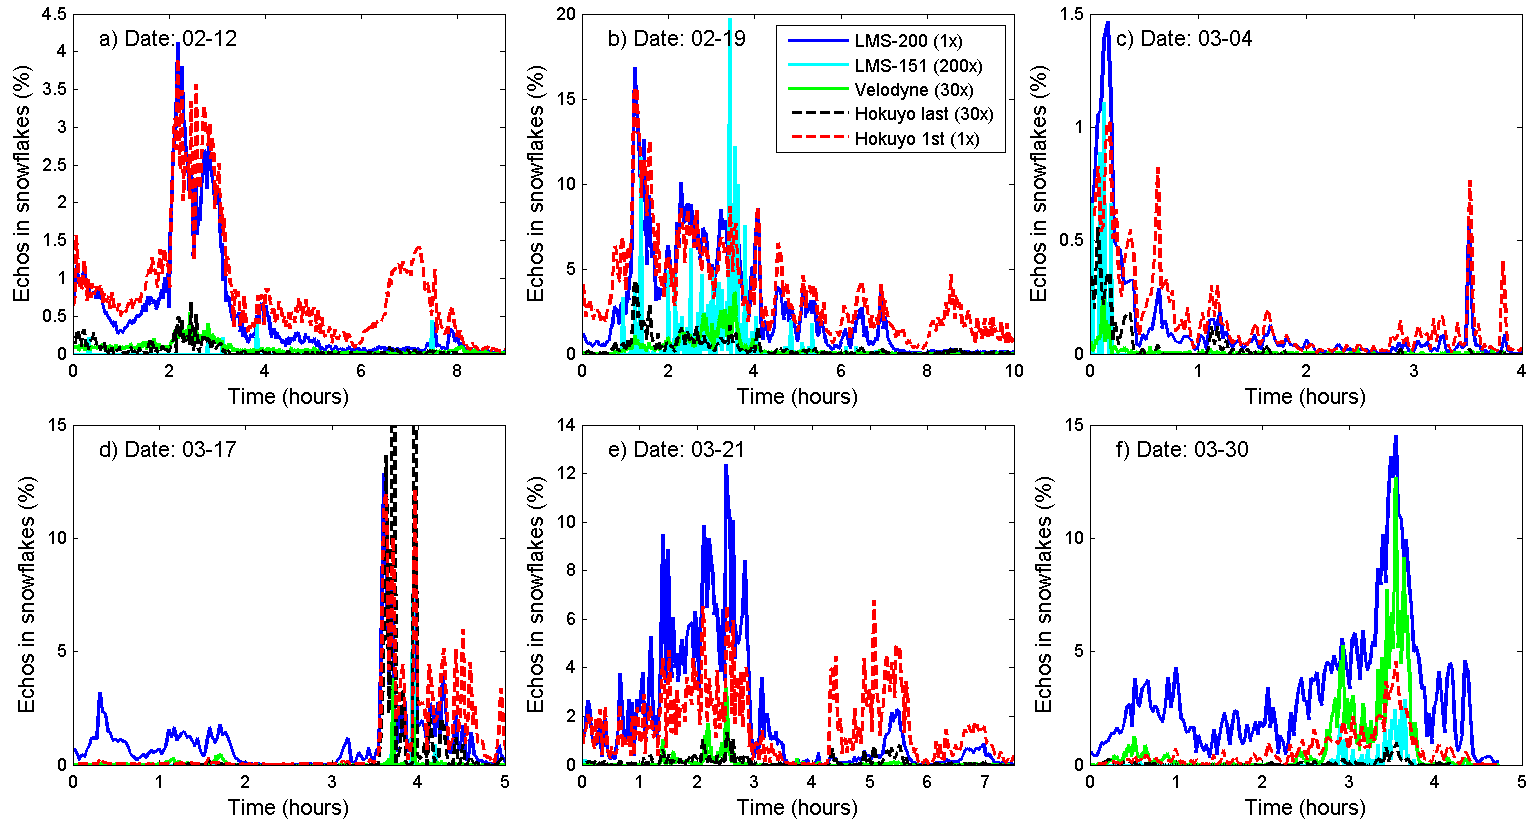
\includegraphics[width=0.98\linewidth]{./img/TimingSnow.png}
    \caption{Temporal evolution of the percentage of echoes coming from the falling snow (range $x<$\SI{5}{\meter}) during the 6 most intense episodes, for all 4 sensors. The data is smoothed by taking statistics for small time windows. Except for the LMS-200 and Hokuyo $1^{st}$ echo, all other sensors statistics have been scaled up (factor in bracket of legend b) for ease of visual comparison. Time is in hour, starting from the beginning of the data capture sequence.}
    \label{fig:TimingSnow}
\end{figure*}


\subsubsection{Hokuyo UTM-30LX-EW}
For the Hokuyo sensor, we resorted to a slightly different approach for comparison, as the device has been designed to return multiple echoes. We thus extracted statistics for two cases: for first and last echo. Statistics for the first echo tells us how sensitive the device is, if one which to detect the presence or absence of falling snow. This information could be used, in turn, to adapt the driving or inform vision algorithms of the presence of particles in the air. Using the last echo ensures that we are able to detect large obstacles such as other vehicle or the snow-covered ground, and used in localization and navigation purposes. In case of the first echo, the device should behave like the LMS-200, and in the second case like the LMS-151 (recall that it was programmed to return the second echo). When looking at Fig.~\ref{fig:TimingSnow}, this is more-or-less the behavior that we see. The Hokuyo's $1^{st}$ echo (blue line) closely track the LMS-200 curves (red dashed line) almost everywhere, with a few exceptions for which we do not have an explanation. The last echo of the Hokuyo tends to reject the falling snow, but not as well as the LMS-151, as it peaked at around 0.5 \% in some episodes. Tab.~\ref{tab:avgRates} shows a similar correlation, but for averages taken over the complete 02-19 dataset. Nevertheless, this difference might not be sufficient to impact algorithms relying on laser data.

\subsubsection{Velodyne HDL-32E}
For all purposes, the behavior of the Velodyne was similar to the Hokuyo's behavior for the last echo. This is seen both in the temporal behavior in Fig.~\ref{fig:TimingSnow} than in the average value displayed in Tab.~\ref{tab:avgRates}.

\subsection{Use of sensitive devices for snowstorm characterization}
(maybe put that in discussion)
A significant side benefit of the more sensitive sensors (LMS-200, Hokuyo UTM-30LX-EW) is that they are capable of recording the temporal evolution of a snowstorm, at a fine-grained level. This is something that is not possible with traditional snow measuring equipment, which can only report accumulation over long period of times. Indeed, for b) we see a pretty steady snowfall from t=1 to t=4 hours, with a peak around t=1.25 hours. This could be helpful in developing temporal models of snowstorms, to be used in a vehicle simulator for example or simply in meteorological studies.

% ========================= Histograms ===================
\subsection{Distribution of echoes in snowflakes, as a function of range $x$}
\label{subsub:Histo}

When modeling a range sensor, one has to have an idea of the probability distribution of certain events (e.g. snowflakes) as a function of the distance to the sensor. Over the years, many researchers have proposed probabilistic models for sensors, notably in Thrun \emph{et al.}~\cite{Thrun:2005:PR:1121596}. In the previous section, we have in some sense estimated the probability for a given sensor S that a snowflake would generate an echo $E_{snowflake}$ given the weather condition $W$, or $P_S(E_{snowflake}|W)$. In this section, we take a closer look at which range $x$ such events would be generated, $P_S(E_{snowflake}|x,W)$. Having such a formulation would allow for a more statistically-sound treatment of the information, such as withing the Bayesian probabilistic framework. To this effect, we use histograms as approximation to the previous distribution. In Fig.~\ref{}, we have plotted these histograms for each of the four sensors. For ease of comparison, these histograms have all been normalized by their total area, as the total count varies widely between the sensors. The numbers in brackets in the legend indicate the fraction of echoes in the snowflakes compared to the total number of data points, for a particular dataset.

%, such as
%\begin{equation}
%p(e|x,w)=p(e|w)p(e|x)
%\end{equation}
%where p(e|x) would be the log-normal distribution and p(e|w) the probability of having snow affecting

The general shape of these histograms is close to a log-normal distribution, with the exception of the LMS-200 for a number of dates (02-12 through 03-17), which seems to follow a sum of two log-normal distributions. This indicate that a simple probabilistic model $P_S(E_{snowflake}|x,W)$ can be derived for these sensors. We break down these distributions into two main regions of interest. The first half (located on the left hand side of the peak) shows an increase in snowflake echoes as a function of the distance $x$. We attribute this phenomenon to the dominant shielding effect of the building from the falling snow. This phenomenon might be absent, to some extent, on an autonomous vehicle. For this reason, we prefer not to discuss it too much in our analysis, as it might not be applicable. The right hand side of the peak shows a gaussian-type exponential decrease of the probability of echos in falling snow. This could be explained by the greatly reduced light intensity (1/$x^2$) of the return, coupled with the decreased light flux/intensity if one assume constant beam size on the way out. These two factors are are illustrated in a cartoon-type model in Fig.~\ref{fig:CartoonModel}. Again, because this is not something we expect to see on a real vehicle, we will not spend too much time on this model.

\begin{figure}[th]
    \centering
    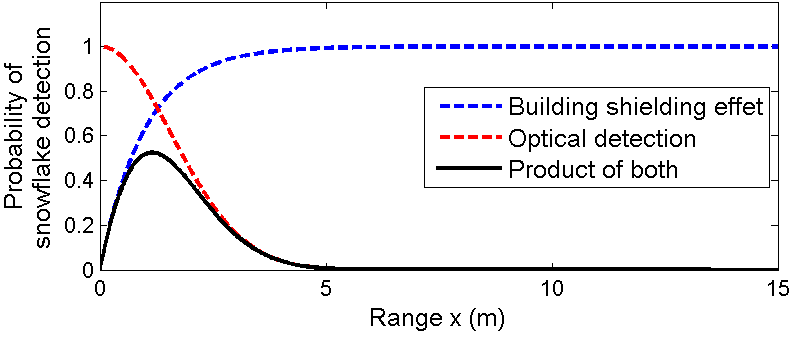
\includegraphics[width=0.97\linewidth]{./img/ShieldingModel.png}
    \caption{Cartoon representation of the interaction between the probability of detecting a snowflake (in red) and the diminution of snowflakes due to the shielding effect of the building (in blue). The black line is the product of the two, and bear a close resemblance to the actual histograms extracted from our data sets.}
    \label{fig:CartoonModel}
\end{figure}

For the LMS-151, the amount of data was not sufficient to draw much conclusion on this distribution except for the fact that there was virtually no events passed 4.


\begin{figure}[th]
    \centering
    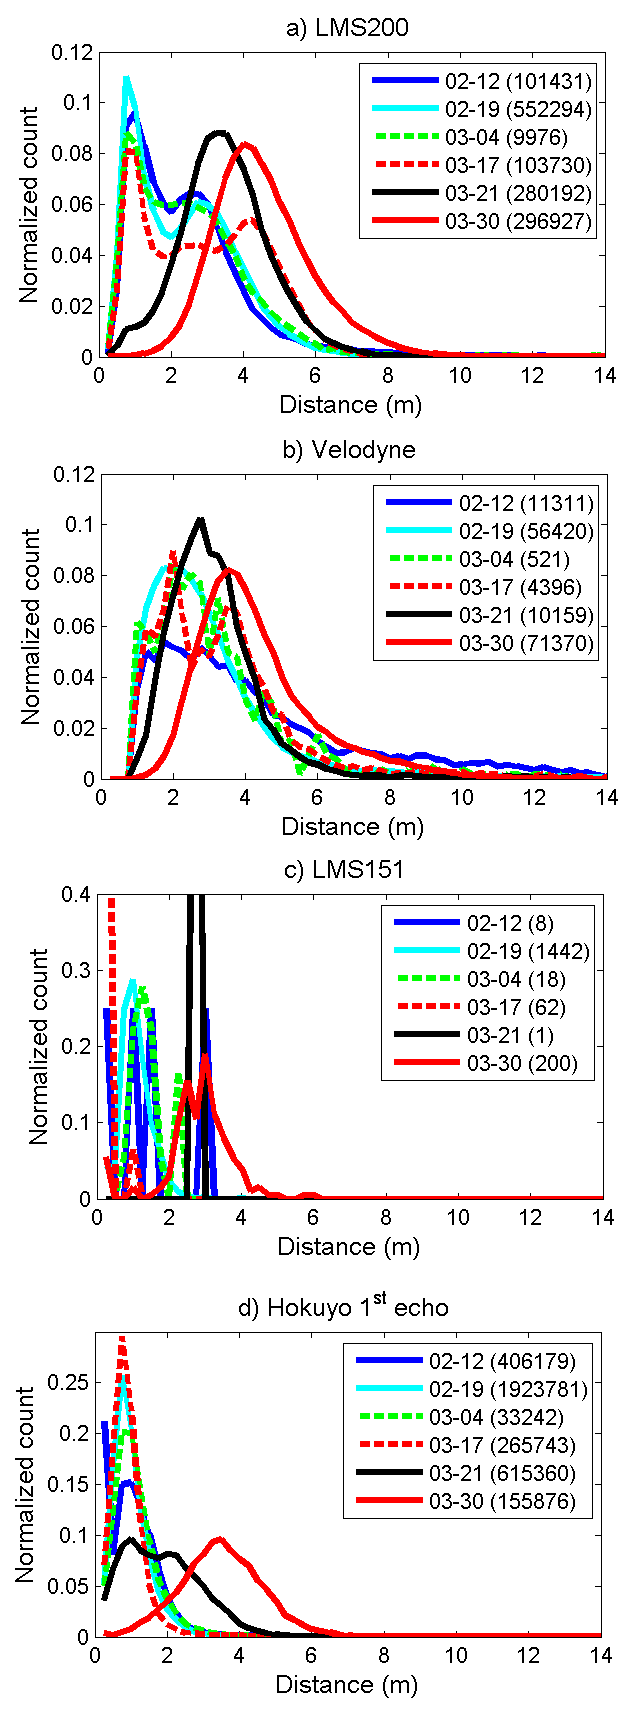
\includegraphics[width=0.80\linewidth]{./img/Histograms.png}
    \caption{Histograms of echoes in falling snow during important snowfall days, as a function of distance $x$ reported by the sensor. Each histogram has been normalized by its area, for ease of comparison. The numbers in brackets are the fraction of data points in the complete data set that correspond to snowflake echoes. Note that for the 03-21 dataset, the LMS151 was not working properly: thus no data is included for that day.}
    \label{fig:Histograms}
\end{figure}

Results show that laser might need to be mounted farther away from the front of the car, so as to avoid the first 1-2 meters that contain significant amount of echos. Or adjust threshold as a function of speed.

\begin{table}[htbp]
    \centering
    \begin{tabular}{|c|c|c|c|c|}
        \hline
        \textbf{LMS-200}       & \textbf{Hokuyo}             & \textbf{Hokuyo}    & \textbf{LMS-151}  & \textbf{Velodyne}  \\
                                        & \textbf{$1^{st}$ echo}   & \textbf{last echo}  &                            & \textbf{HDL-32E}  \\\hline
                 2.67\%            &           3.55\%                &       0.0113\%      &       0.00178\%     &  0.0100\%  \\\hline
    \end{tabular}
    \caption{Average snowflakes echos for the 02-19 data set, per sensor.}
    \label{tab:avgRates}
\end{table}

% ======================= Sunlight =====================
\subsection{Impact of sunlight on Hokuyo}

Note that however there was instance (daytime with sun) where the sensor didn't return echoes at all. We suspect that this is sue to the fact that the power level used. More on this in a following subsection.

% ======================= Sunlight =====================
\subsection{Discussion}
It seems that the majority of the impact of falling snow is for the first 5-6 meters. For near distance, this would impact the collision/obstacle avoidance. However, the problem at long range does not seem to happen, at least based on extrapolating from our data set.

Open question such as how the maximum range is affected by the snow.

